\section{Résultats de couverture (Jacoco)}
\noindent
Comme mentionné précédemment, nous utilisons \textbf{JaCoCo} pour mesurer l'efficacité de la couverture de notre suite de tests. 

\subsection{Résultats de la couverture}
\begin{figure}[H]
    \centering
    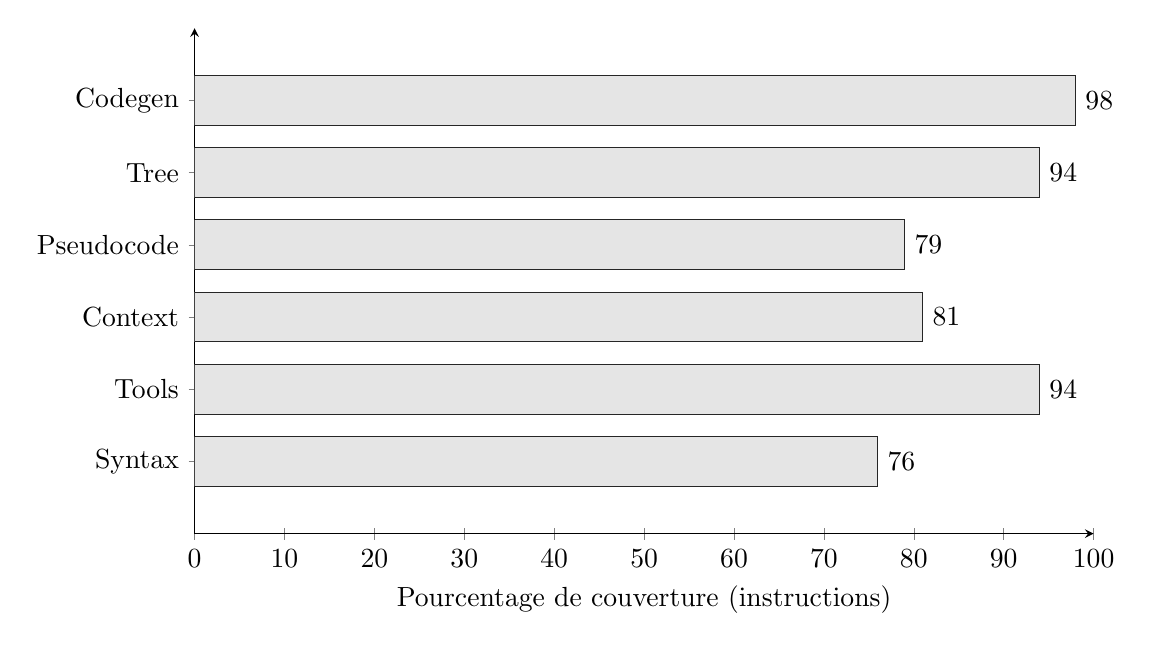
\begin{tikzpicture}
        \begin{axis}[
            xbar,
            width=13cm,
            height=8cm,
            xmin=0, xmax=100,
            xlabel={Pourcentage de couverture (instructions)},
            symbolic y coords={Syntax,Tools,Context,Pseudocode,Tree,Codegen},
            ytick=data,
            nodes near coords,
            nodes near coords align={horizontal},
            axis x line=bottom,
            axis y line=left,
            bar width=18pt,
            enlarge y limits=0.2,
        ]
            \addplot[
                fill=gray!20,
                draw=gray!30!black
            ] coordinates {
                (76,Syntax)
                (94,Tools)
                (81,Context)
                (79,Pseudocode)
                (94,Tree)
                (98,Codegen)
            };
        \end{axis}
    \end{tikzpicture}
    \caption{Couverture JaCoCo par paquetage (en pourcentage d'instructions)}
\end{figure}



\noindent
\textit{NB : Les rapports détaillés sont générés dans \texttt{target/site/jacoco/index.html} après chaque exécution de \texttt{mvn verify -Djacoco.skip=false}.}

\subsection{Analyse des résultats}

\paragraph*{Fiabilité de la couverture} \mbox{} \\
\noindent
Paradoxalement, le package \texttt{codegen} affiche la meilleure couverture (98\%), alors que c'est la phase ou nous avons rencontré le plus d'erreurs après le rendu du projet. Cela s'explique notamment par le fait que ce package ne contient que les \texttt{Managers} et montre ainsi qu'il n'y a pas de méthodes ou de champs non utilisés même si cela ne garantit pas que la logique interne fonctionne correctement.

\paragraph*{Rigueur de l'analyse contextuelle} \mbox{} \\
\noindent 
Le package \texttt{context} (81\%) et les outils associés (\texttt{tools} à 94\%) démontrent que notre stratégie de tests unitaires et fonctionnels a réussi, couvrant la quasi-totalité des vérifications de types et de la gestion de la table des symboles.

\paragraph*{Zones d'amélioration} \mbox{} \\
\noindent 
Le package \texttt{syntax} (76\%) affiche un score plus bas, ce qui est structurel : une partie du code est générée par ANTLR et correspond à des chemins de récupération d'erreurs syntaxiques complexes qu'il est difficile de provoquer intégralement. De même, malgré les efforts, les scores correspondant aux "branches manquées" sont plus faible ce qui indique que nous aurions pu tester d'avantage tous les cas qu'ils soient positifs ou négatifs.

\noindent
En définitive, le compilateur atteint une couverture globale de 83\% des instructions couplée à une validation de 71\% des branches logiques ce qui témoigne d'une stratégie de test rigoureuse et fiable.